\section{Results}
Each version of the program was tested on the Xeon PHI machine, the tests were done with 10 generation and 20000 chromosomes and considering [500, 1000, 2000] nodes in the graph. As we can see from the curves, a good speedup is obtained with the first 50 threads because genetic algorithm are generally highly parallelizable algorithms. But as expected from the theory, after spawning more than 100 threads the overhead taken to set up and coordinate the computation is higher than the parallelism benefits obtained by adding threads. Surely with a bigger graph as input, the speedup curve would be increasing even with more than 100 threads. 

\subsection{Speedup curves}
\begin{figure}[H]
	\centering
\begin{minipage}[t]{0.50\linewidth}
	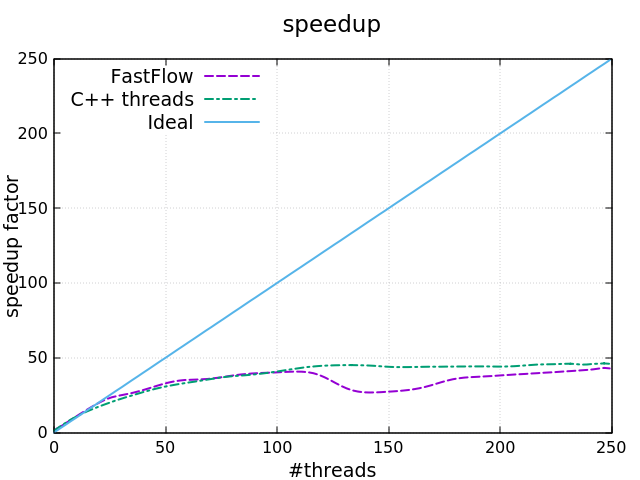
\includegraphics[width=\linewidth]{benchmark/curves/speedup_standard_2000_20000.png}
	\vspace{0.2em}
	%\subcaption{} 
\end{minipage}%
\begin{minipage}[t]{0.50\linewidth}
	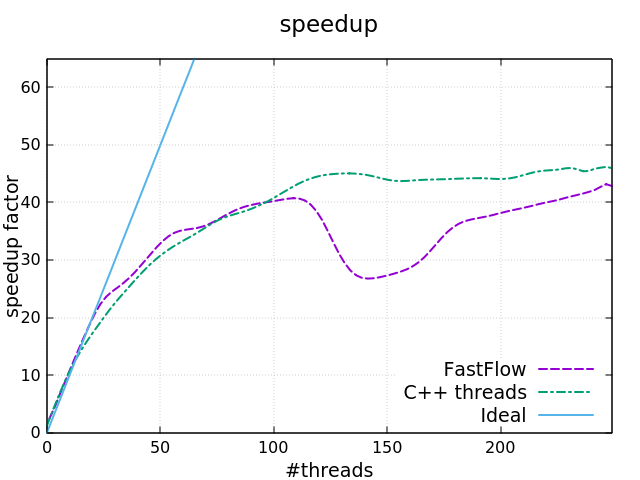
\includegraphics[width=\linewidth]{benchmark/curves/speedup_zoom_2000_20000.png}
	%\subcaption{}
\end{minipage}
\caption{Speedup 2000 nodes}\label{fig:speedup2000}
\end{figure}
\begin{figure}[H]
	\centering
	\begin{minipage}[t]{0.50\linewidth}
		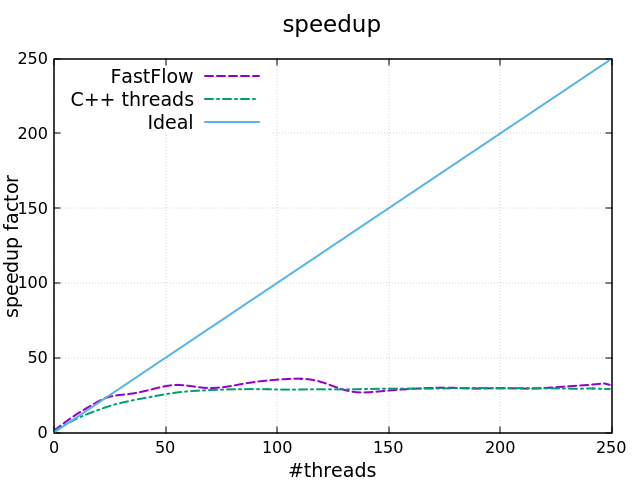
\includegraphics[width=\linewidth]{benchmark/curves/speedup_standard_1000_20000.png}
		\vspace{0.2em}
		%\subcaption{} 
	\end{minipage}%
	\begin{minipage}[t]{0.50\linewidth}
		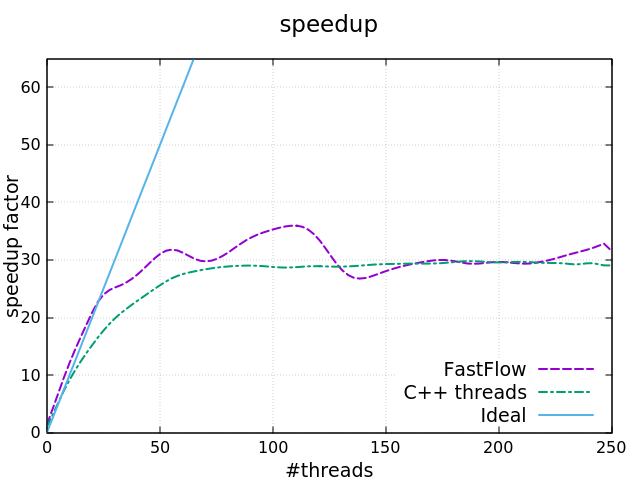
\includegraphics[width=\linewidth]{benchmark/curves/speedup_zoom_1000_20000.png}
		%\subcaption{}
	\end{minipage}
	\caption{Speedup 1000 nodes}\label{fig:speedup1000}
\end{figure}

\begin{figure}[H]
	\centering
	\begin{minipage}[t]{0.50\linewidth}
		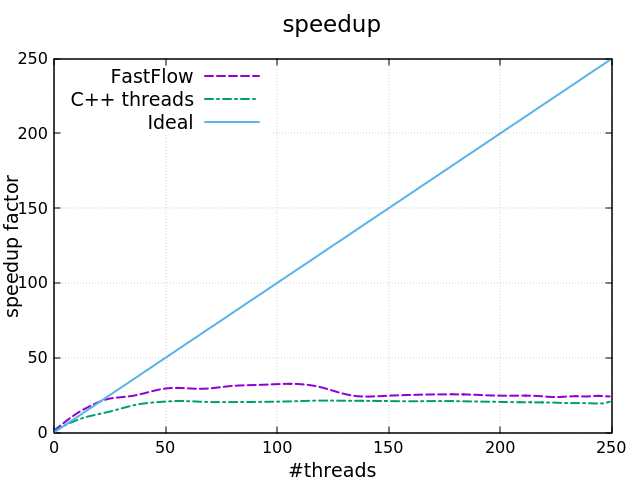
\includegraphics[width=\linewidth]{benchmark/curves/speedup_standard_500_20000.png}
		\vspace{0.2em}
		%\subcaption{} 
	\end{minipage}%
	\begin{minipage}[t]{0.50\linewidth}
		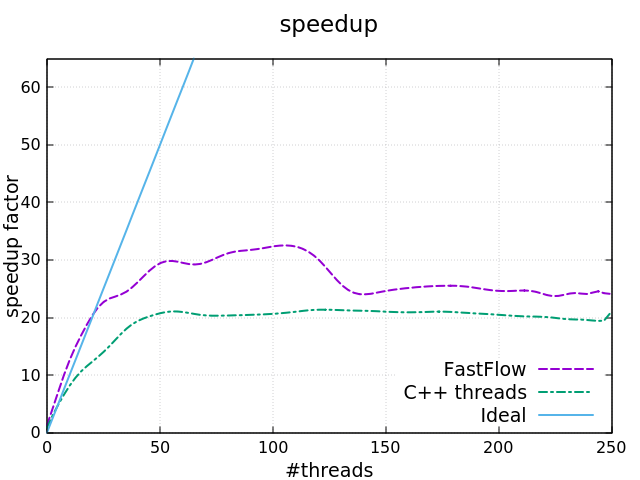
\includegraphics[width=\linewidth]{benchmark/curves/speedup_zoom_500_20000.png}
		%\subcaption{}
	\end{minipage}
	\caption{Speedup 500 nodes}\label{fig:speedup500}
\end{figure}

\subsection{Scalability curves}
\begin{figure}[H]
	\centering
\begin{minipage}[t]{0.50\linewidth}
	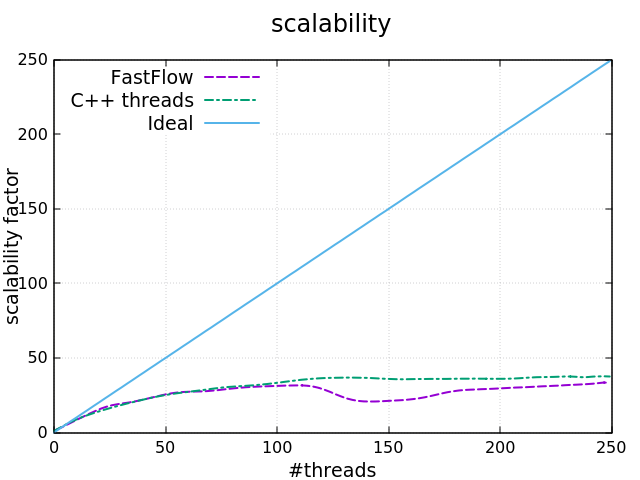
\includegraphics[width=\linewidth]{benchmark/curves/scalability_standard_2000_20000.png}
	\vspace{0.2em}
	%\subcaption{} 
\end{minipage}%
\begin{minipage}[t]{0.50\linewidth}
	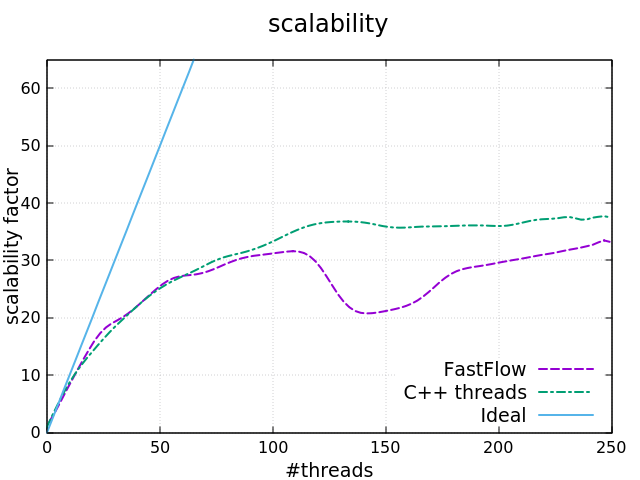
\includegraphics[width=\linewidth]{benchmark/curves/scalability_zoom_2000_20000.png}
	%\subcaption{}
\end{minipage}
\caption{Scalability 2000 nodes}\label{fig:scalability2000}
\end{figure}

\begin{figure}[H]
	\centering
	\begin{minipage}[t]{0.50\linewidth}
		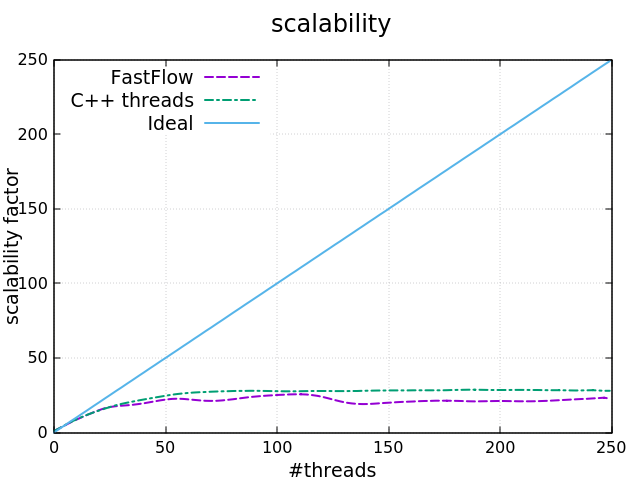
\includegraphics[width=\linewidth]{benchmark/curves/scalability_standard_1000_20000.png}
		\vspace{0.2em}
	%	\subcaption{} 
	\end{minipage}%
	\begin{minipage}[t]{0.50\linewidth}
		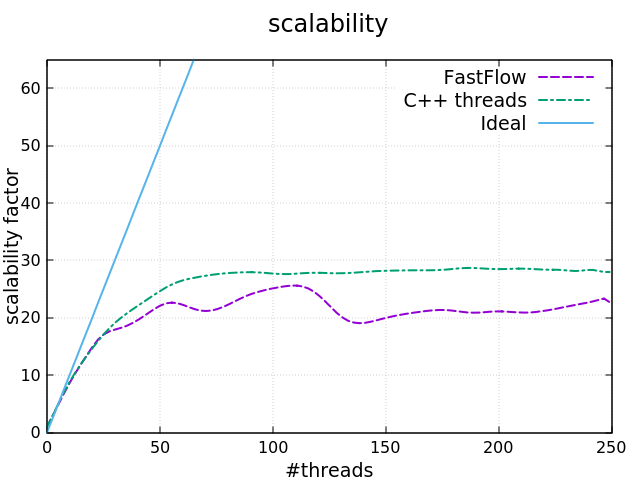
\includegraphics[width=\linewidth]{benchmark/curves/scalability_zoom_1000_20000.png}
	%	\subcaption{}
	\end{minipage}
	\caption{Scalability 1000 nodes}\label{fig:scalability2000}
\end{figure}

\begin{figure}[H]
	\centering
	\begin{minipage}[t]{0.50\linewidth}
		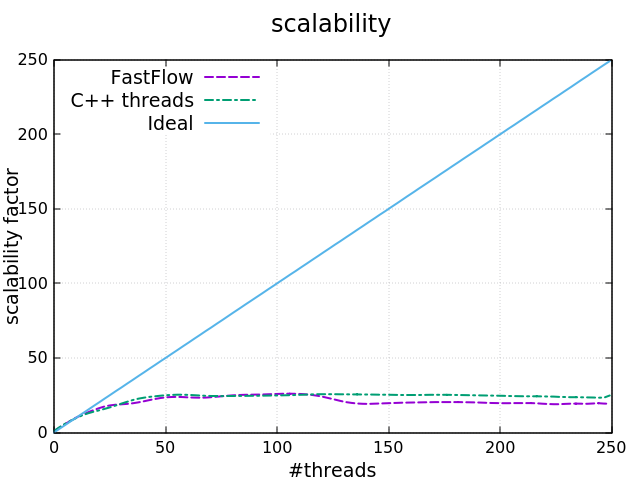
\includegraphics[width=\linewidth]{benchmark/curves/scalability_standard_500_20000.png}
		\vspace{0.2em}
	%	\subcaption{} 
	\end{minipage}%
	\begin{minipage}[t]{0.50\linewidth}
		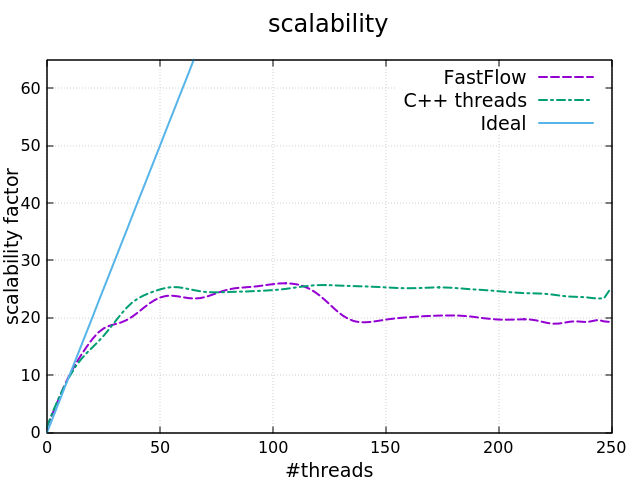
\includegraphics[width=\linewidth]{benchmark/curves/scalability_zoom_500_20000.png}
	%	\subcaption{}
	\end{minipage}
	\caption{Scalability 500 nodes}\label{fig:scalability2000}
\end{figure}